\subsubsection{Creazione e gestione dei task}
Per la creazione di un task si procede nel seguente modo:
\begin{itemize}
    \item Accesso alla task list relativa al progetto di interesse identificata con il nome dello stesso.
    \item Creazione di un nuovo task.
    \item Il Responsabile di Progetto può decidere si suddividerlo in sotto-task da assegnare a membri del gruppo differenti.
\end{itemize}
\subsubsection{Gestione dei ticket}
La vita di ogni ticket viene presentata nel seguente diagramma:

\begin{figure}[h!]
  \begin{center}
  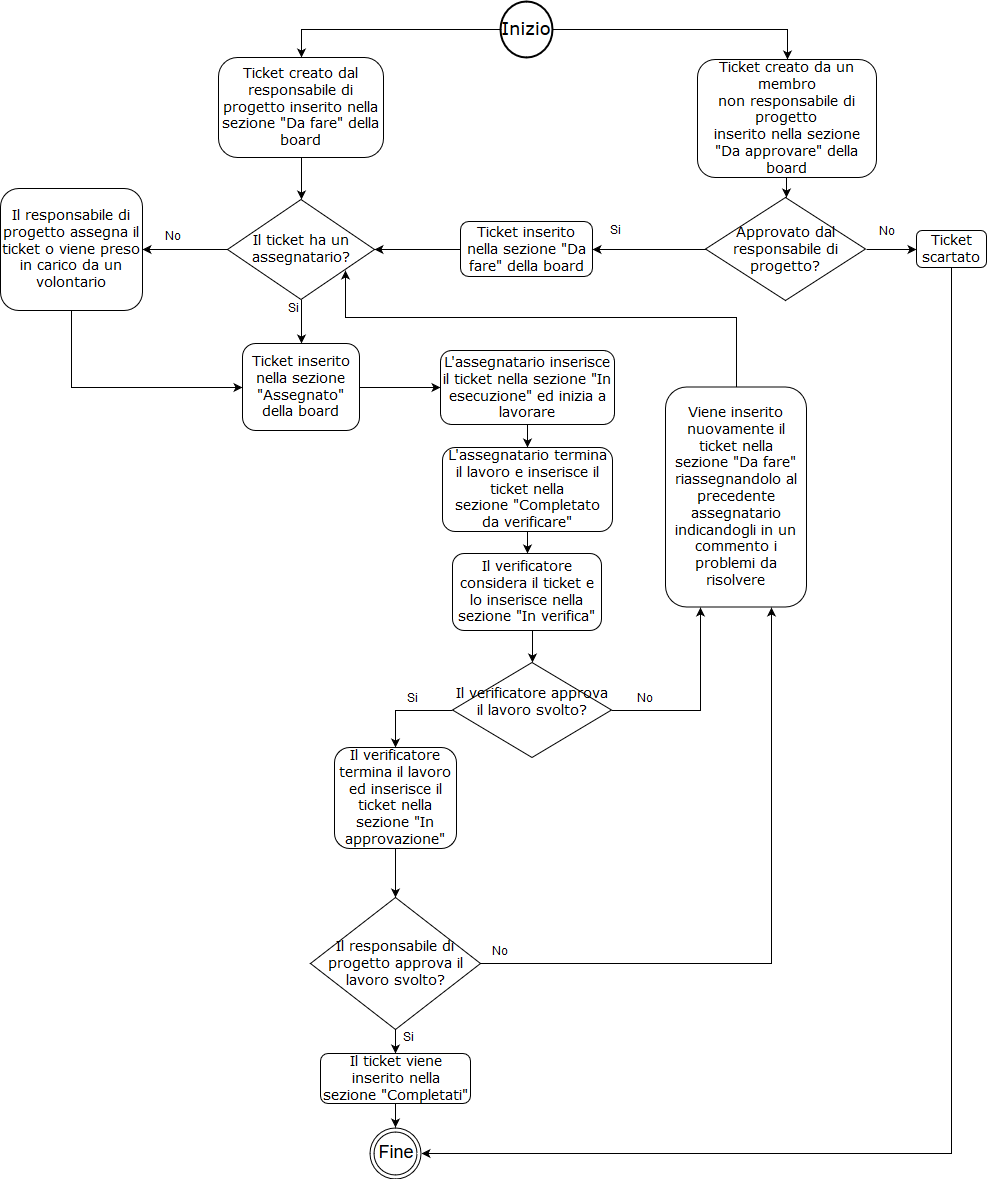
\includegraphics[scale=0.50]{immagini/Dt.png}
  \caption{Diagramma del ciclo di vita di un ticket}
  \end{center}
\end{figure}

\newpage

\subsubsection{Stesura del consuntivo}
L'operazione di stesura del consuntivo viene eseguita dal Responsabile di Progetto nel seguente modo:
\begin{itemize}
    \item Esporta da \citgl{Gantt project} un file in formato \citgl{Microsoft Excel} che indica le ore rendicontate nella fase corrente;
    \item Accede al \citgl{Foglio di Google} presente nel \citgl{Google Drive} associata alla mail del gruppo con relativo template e ne fa una duplicazione;
    \item Inserisce le ore rendicontate nelle apposite celle ottenendo la differenza con quelle preventivate;
    \item Riporta i valori ottenuti nel Piano di Progetto;
    \item Crea una tabella che, elaborando i dati derivanti dalla differenza tra le ore rendicontate e quelle preventivate, trova il budget effettivo rispetto a quello previsto;
    \item Infine con l'elaborazione di questi dati crea una valutazione complessiva del lavoro.
\end{itemize}
Per il periodo che precede la revisione RR ci si ferma al punto 3 senza ricavarne la differenza in quanto le ore preventivate non sono presenti. Successivamente ad ogni revisione sarà aggiornato il Piano di Progetto con i dati ottenuti.

